%%%%%% CMB-S4 Lensing Chapter  %%%%%%%%%%%%%%%%
 
\chapter{CMB Lensing}
%\renewcommand*\thesection{\arabic{section}}


\def\nnu{N_{\mathrm eff}}
\def\gtrsim{\raise-.75ex\hbox{$\buildrel>\over\sim$}}
%%%%%%%%%%%%%%%%%%%%%%%%%%%%%%%%%%%%%%%%%%%%%%%%%%%%%%%%%%%
%%%%%%%%%%%%%%%%%%%%%%%%%%%%%%%%%%%%%%%%%%%%%%%%%%%%%%%%%%%
%%%%%%%%%%%%%%%%%%%%%%%%%%%%%%%%%%%%%%%%%%%%%%%%%%%%%%%%%%%
%%%%%%%%%%%%%%%%%%%%%%%%%%%%%%%%%%%%%%%%%%%%%%%%%%%%%%%%%%%

\section{Introduction to CMB Lensing}

Measuring the deflection of microwave background light by the gravitational influence of matter along its path through the Universe is a powerful way to determine the properties of neutrinos and dark energy and constrain inflationary signals.  As CMB photons travel to us from the surface of last scattering their paths are slightly altered by the gravity of the mass distribution through which they pass.  These gravitational lensing deflections lead to a remapping of the primordial CMB sky, and this remapped sky is what we observe today.  Measuring the properties of this lensing deflection is interesting for two reasons:\\


$\bullet$ CMB lensing encodes a wealth of statistical information about the entire large-scale structure distribution, which in turn encodes information on the properties of neutrinos and dark energy.\\


$\bullet$ CMB lensing obscures our view of the primordial Universe, limiting our power to constrain inflationary signals; removing this lensing noise more cleanly brings the early Universe and any inflationary signatures into sharper focus.\\

The lensing of the CMB can be measured by relying on the fact that the statistical properties of the primordial CMB are well known.  Lensing changes these well-understood statistical properties, breaking statistical isotropy and thus correlating formerly independent modes of the CMB temperature and polarization fields.  Precisely measuring these correlations can be used to map out the lensing deflections and the projected large-scale structure that caused them, as discussed in more detail in Section \ref{kappaMap}.

The power spectrum of the lensing deflection map is sensitive to any physics that modifies how structure grows, such as dark energy, modified gravity, and the masses of neutrinos.  In Section \ref{kappaPower}, we discuss how the lensing how the lensing power spectrum is measured, and in Section \ref{params}, we give parameter forecasts combining CMB power spectrum and CMB lensing power spectrum measurements.   Another key application of lensing as a signal is the comparison of CMB lensing maps with the distribution of galaxies and optical weak lensing shear maps.  This can give insights  via calibration of systematic effects as well as enhanced dark energy constraints. Cross-correlation science with CMB lensing maps is discussed in Section \ref{cross}.

However, lensing is not only a signal that probes the cosmological mass distribution. It is also source of noise in measurements of a primordial B-mode polarization signal, which limits studies of inflation and the early Universe. With precise measurements, of lensing, however, this limiting source of noise can be removed, in a procedure known as delensing. This procedure, which will be crucial for the lensing-noise dominated B-mode polarization measurements from CMB-S4, is described in Section \ref{delens}.  We discuss systematics from astrophysical and instrumental effects that can inpact the lesning signal as well as ways to mitigate them in Section \ref{syst}.  Section \ref{require} describes the instrument, survey, and simulation requirements for CMB-S4 to maximize the science gain from CMB lensing measurements.


%%%%%%%%%%%%%%%%%%%%%%%%%%%%%%%%%%%%%%%%%%%%%%%%%%%%%%%%%%%
\section{Measuring CMB Lensing}

\subsection{Constructing a Lensing Map}\label{kappaMap}

A map of the CMB lensing deflection field is a direct probe of the projected matter distribution that exists in the observable Universe. This lensing map is a fundamental object for nearly all areas of CMB lensing science: it is used to measure the lensing power spectrum, measure cross correlations between CMB lensing and external data sets, and to de-lens maps of the B-mode polarization.  

\begin{figure}[h]
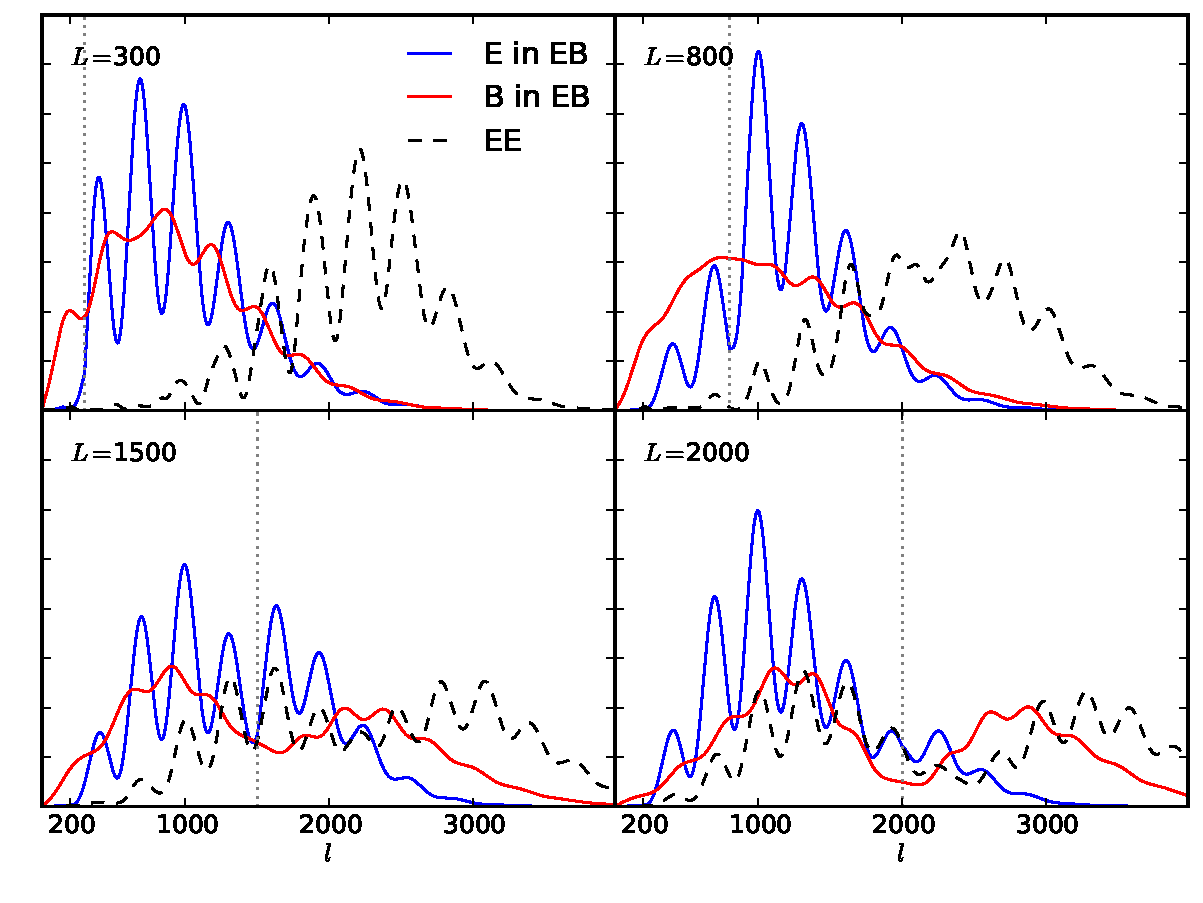
\includegraphics[width=0.95\textwidth]{CMBLensing/signal_contribs.pdf}
\caption{}
\end{figure}

To date, all maps of the lensing field have been constructed using the quadratic estimator by Hu \& Okamoto 2002.  This estimator uses information about the off-diagonal mode-coupling in spherical harmonic space that lensing induces to reconstruct the deflection field.  An estimate for the amount of lensing on a given scale is obtained by averaging over pairs of CMB modes in harmonic space separated by this scale (cite).  The high angular resolution of CMB-S4 improves upon the Planck measurement by increasing the number of CMB modes imaged on scales smaller than the Planck beam.  Imaging CMB modes between $l=2000$ and 3000, which can be achieved with CMB-S4 yields considerable gain in the accuracy of the lensing power spectrum measurement (cite).    

\begin{figure}[h]
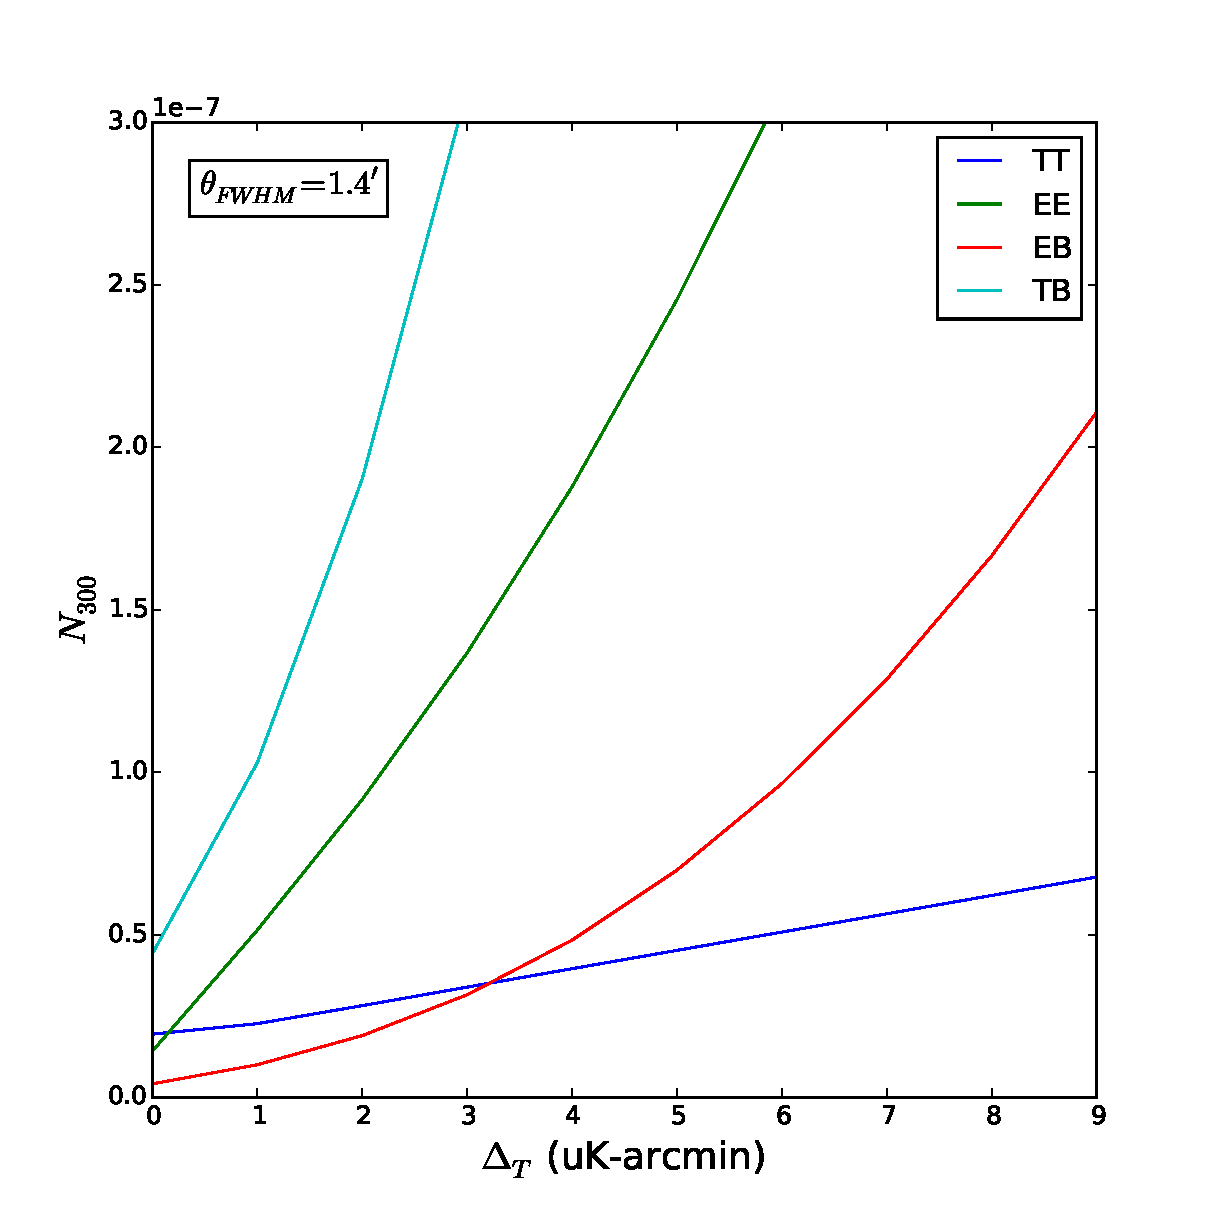
\includegraphics[width=0.45\textwidth]{CMBLensing/ell300_1_40.pdf}
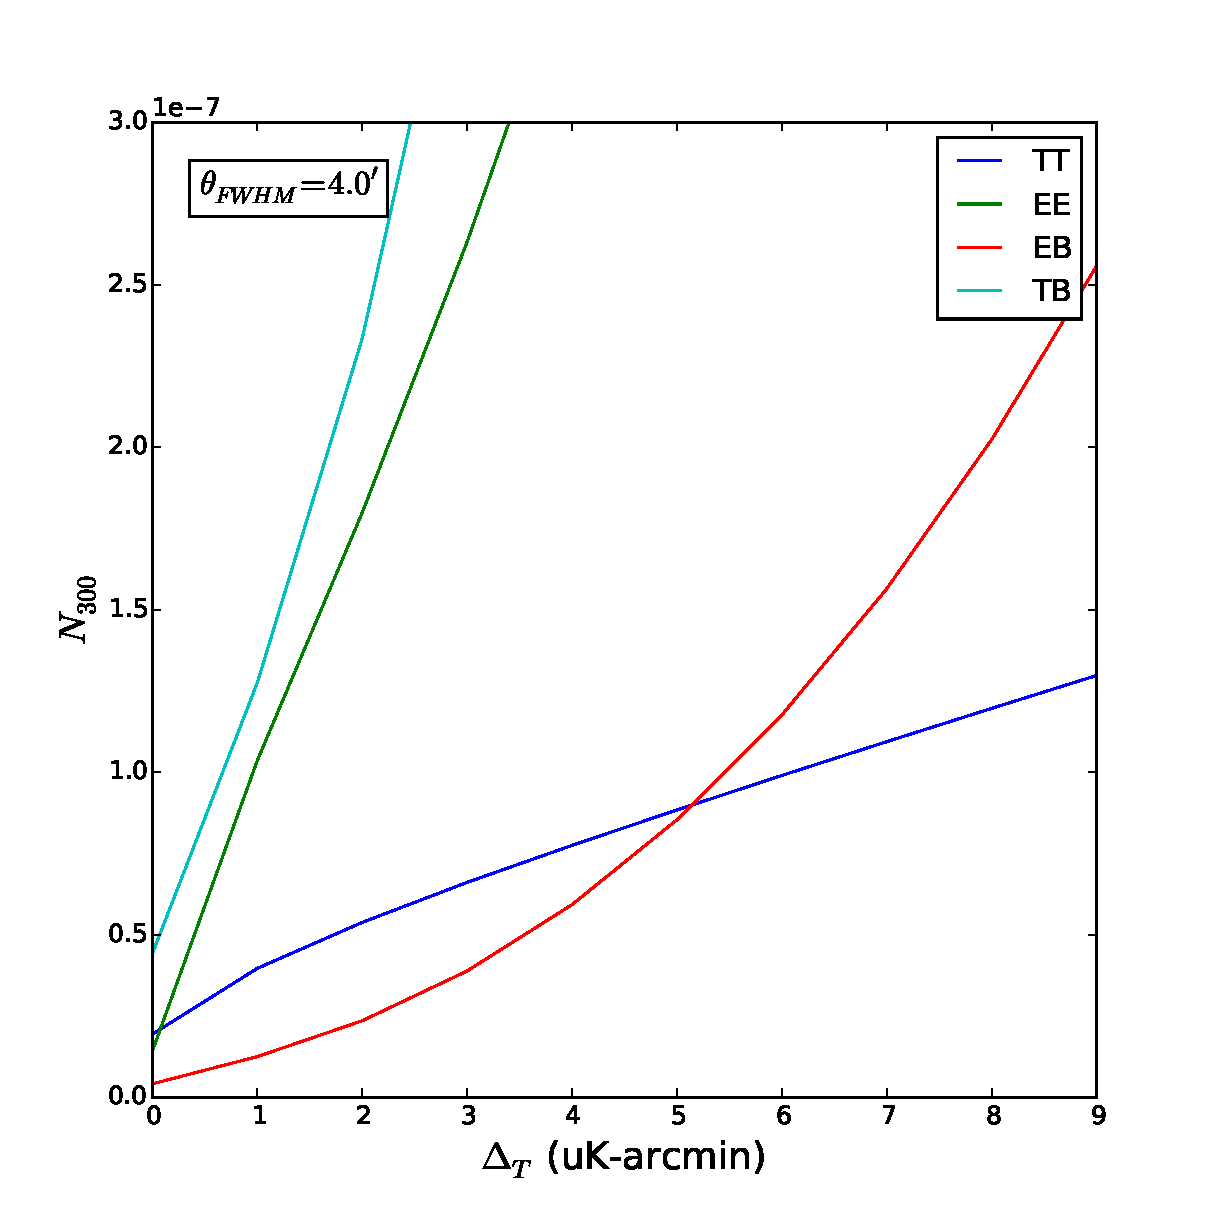
\includegraphics[width=0.45\textwidth]{CMBLensing/ell300_4_00.pdf}
\caption{Noise per mode in the lensing field for different lensing estimators at $L = 300$.  Left panel is for 1.4 arcmin resolution, and right panel is for 4 arcmin resolution.  For a 1.4 and 4 arcmin resolution experiment, the EB polarization estimator yields lower noise than the temperature estimator, below 3uk-arcmin and 5uk-arcmin noise in temperature respectively.}
\end{figure}


The increased sensitivity of CMB-S4 also puts CMB lensing measurements in a new regime for two reasons.  The first is that to date all CMB lensing results have had their signal-to-noise dominated by lensing reconstructions based on CMB temperature data (cite).  While first results using CMB polarization have been obtained (cite), the unprecedented sensitivity of CMB-S4 will allow the bulk of lensing signal-to-noise to be derived from CMB polarization data, where atmospheric noise and systematic biases from astrophysical foregrounds are greatly reduced.  The second reason CMB lensing measurements will enter a new regime with CMB-S4 is becasue the low instrument noise of CMB-S4 will allow use of an iterative delensing technique.  With this iterative technique, the quadratic estimator operation can be repeated many times on B-mode maps resulting in higher fidelity lensing maps than with a single estimator operation (cite), as discussed in more detail in Section \ref{delens}.   





\subsection{Lensing Power Spectrum}\label{kappaPower}

The power spectrum of reconstructed CMB lensing maps is a measure of the matter power spectrum integrated over redshift.  The lensing power spectrum has a broad redshift response kernel, with most of the contribution coming from $z\sim 1-5$, with a peak at $z\sim 2$ (cite).  
%(Figure \ref{fig:cmblens_kernel}).  
Most of the scales probed by the lensing power spectrum are on large enough scales that they are mainly in the linear regime.  As such, the lensing power spectrum is sensitive to physics which affects the growth of structure on large scales and at high redshift, such as the mass of the neutrinos. 

The latest measurements of the CMB lensing autospectrum, as of early 2016, are shown in Figure \ref{CMBLensPower}. The first detections were obtained by the Atacama Cosmology Telescope (ACT; \cite{das/etal/2011}) and South Pole Telescope  (SPT; \cite{vanengelen/etal/2012}) teams, who analyzed maps of several hundreds of square degrees yielding precisions on the lensing power spectrum of approximately 25\% and 18\% respectively.  The Planck collaboration has since provided all-sky lensing maps whose precision on the power spectrum amplitude is approximately 4\% in the 2013 data release and 2.5\% in the 2015 data release.  The first detections of the lensing autospectrum using CMB polarization, which is ultimately a more sensitive measure of lensing for low-noise maps,  have also been obtained \cite{story/etal/2013, polarbear/lensing//2014}.

\begin{figure}[h]
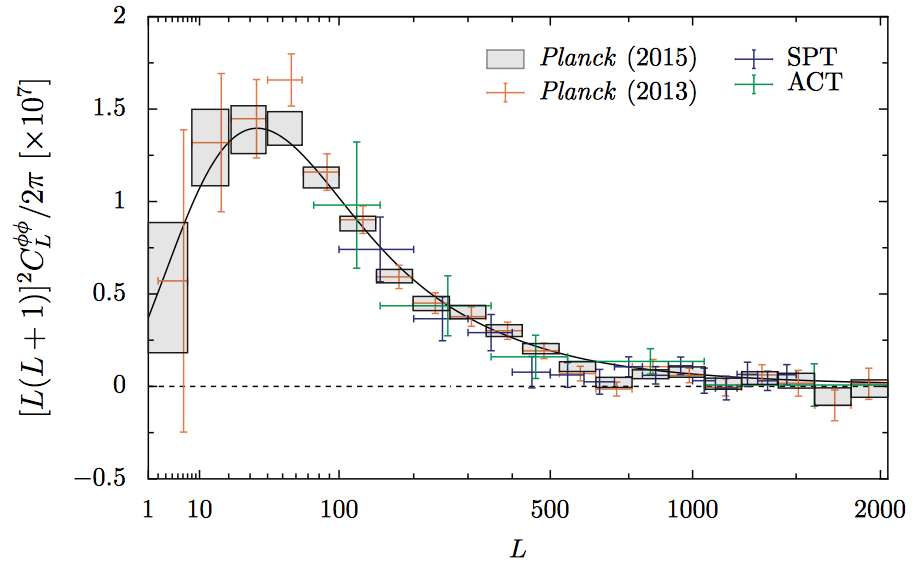
\includegraphics[width=0.95\textwidth]{CMBLensing/CMBLensPower.png}
\caption{test}
\label{CMBLensPower}
\end{figure}

In spite of the rapid improvement in these measurements over the period of just a few years, no part of the CMB lensing autospectrum is yet sample variance limited.  The  power spectrum of the noise in the CMB lensing reconstruction  in the 2015 Planck data release is approximately equal to the lensing power spectrum at its peak of $L \sim 40$, but smaller scales are noise-dominated.  Lensing reconstructions from  ground-based surveys are signal-dominated below $L \sim 200$ and noise-dominated on smaller scales.  However, they have been obtained over relatively small sky areas of several hundreds of degrees. A ground-based survey such as CMB-S4, with wide sky coverage, low-noise, and high resolution, will provide a sample-variance-limited measurement to scales below $L \sim 1000$ (see Figure \ref{Neutrinos}).  
 


\begin{figure}[h]
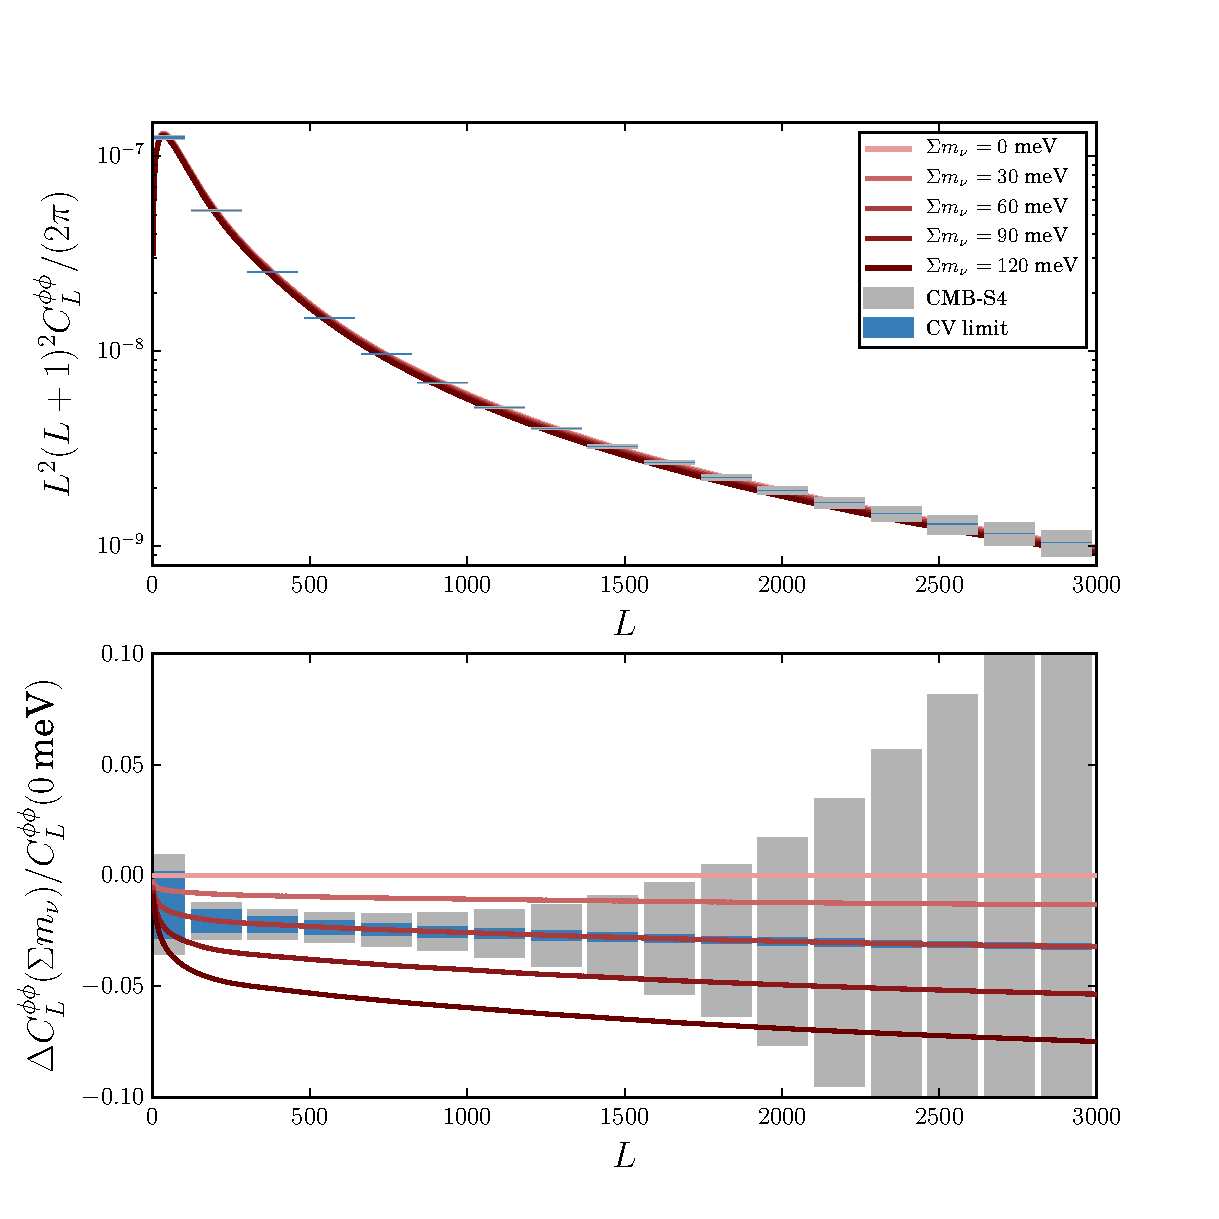
\includegraphics[width=0.95\textwidth]{CMBLensing/s4errors.pdf}
\caption{test}
\label{Neutrinos}
\end{figure}

 
 
Such a measurement holds the promise to qualitatively improve our understanding of cosmology.  While the cosmological parameters describing the standard Lambda-Cold Dark Matter model have been precisely measured \cite{planckpapers}, extensions to this model can be constrained by including growth or geometrical information at a new redshift.  From the redshifts probed by CMB lensing, extensions to the standard model such as a non-minimal mass for the sum of the neutrinos, a dark energy equation of state deviating from the vacuum expectation, and a non-zero curvature of the Universe can all be probed to much higher precision than with the primordial CMB alone. 



%-brief aside: biases\\

%-brief summary of how neutrinos affect large scale structure with plots \\

%-why lensing is a particularly good way of probing neutrinos\\



\subsection{Parameter Forecasts with Lensing}\label{forecast}

Since CMB lensing is a sensitive probe of the matter power spectrum, CMB lensing measurements added to measurements of the primordial CMB power spectrum serve to significantly tighten parameter constraints.  In particular, measurements of the CMB lensing autospectrum yield tight constraints on neutrino properties, such as the number of neutrinos species ($N_{\rm{eff}}$) and the sum of the masses of the neutrinos ($\sum {m_\nu}$).  We present forecasts for $\sigma(N_{\rm{eff}})$ and $\sigma(\sum {m_\nu})$ for CMB-S4 below.  

Cross correlations of CMB lensing maps with maps of galaxy density and galaxy shear can further provide tight constraints on the dark energy equation of state ($w$) and modified gravity as presented in Section \ref{crossForecast}.  Delensing B-mode polarization maps from CMB-S4 can also give strong constraints on the tensor-to-scalr ratio ($r$) from inflationary primordial gravity waves, as discussed more fully in Section \ref{delensForecast}.

\begin{figure}[h]
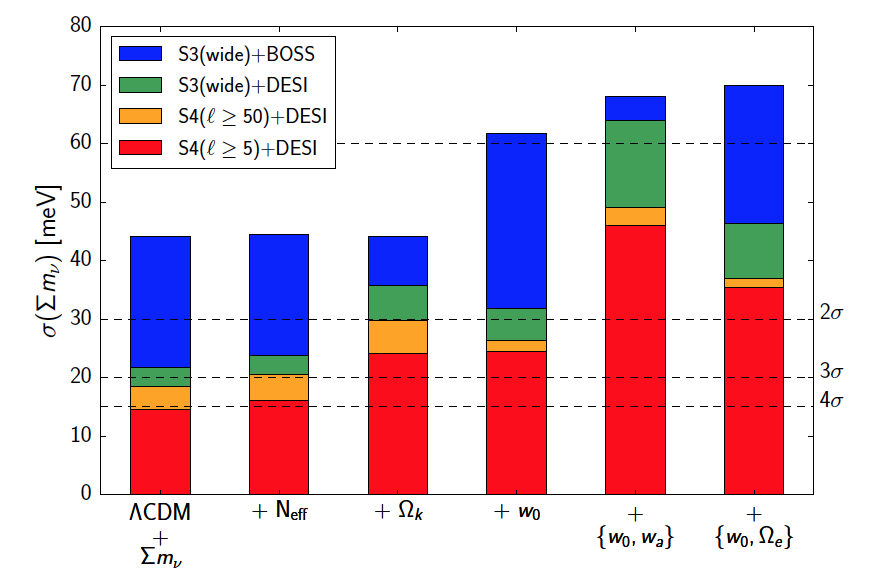
\includegraphics[width=0.95\textwidth]{CMBLensing/Allisonetal.png}
\caption{place holder from Allison et al 2015}
\label{nuForecasts}
\end{figure}

%-forecasting assumptions for noise etc\\
%-power spectrum forecasts incl s/n\\
%-results for neutrinos\\
%-robustness and comparison with other probes\\

For these forecasts, we assumed...

\section{Cross Correlations with CMB Lensing}\label{cross}

A useful application of CMB lensing measures is in cross-correlation with other probes of large-scale structure.  This can yield higher detection significances, can be less prone to systematic effects, and given the generally lower redshift distribution of the other tracer, can more directly probe the evolution of dark energy.


\subsection{CMB Lensing Cross Galaxy Density}


Very high S/N will be possible with S4 and various surveys.   Different dependence on bias factors ($b^2$ vs $b$.  Can also be done in tomography.

-In principle, alternative route to measuring neutrino masses (with LSST galaxies: 50 meV -- Pearson \& Zahn 2013), but biases need to be understood as functions of z and k/M.  

\subsection{CMB Lensing Cross Galaxy Shear}



\subsubsection{Forecasts for CMB Lens Cross Galaxy Density and Galaxy Shear}\label{crossForecast}

0.3\% amplitude constraint with S4xLSST.  Also, EUCLID, WFIRST.

Applications:

-Mass tomography -- CMB can be used as highest-redshift plane in tomographic lensing studies serving as an anchor in the matter-dominated era for dark energy studies

-In principle, calibrating multiplicative bias from cosmic shear (Valinotto 2011).  Will LSST x S4 be good enough to help with LSST auto?

-Can also add crosses with galaxy distribution (3x further improvement -- Das, Errard, \& Spergel 2014)

-Can constrain optical weak lensing multiplicative bias.

-Possibly help with calibrating WL intrinsic alignments?

\subsection{Halo Lensing}


The abundance of galaxy clusters as a function of mass and redshift provides a direct handle on the growth of matter perturbations and consequently, on the equation of state of Dark Energy. Clusters can be identified internally in CMB maps through their wavelength-dependent imprint via the thermal Sunyaev-Zeldovich (tSZ) effect. However, the scaling relations between the tSZ observable and the true mass of the cluster possess intrinsic scatter due to the complex gas physics producing the tSZ effect. Calibration of this mass uncertainty is currently the dominant systematic for extracting Dark Energy constraints from cluster abundance measurements. Weak lensing of sources behind the galaxy cluster is a promising method for mass calibration since it is directly sensitive to the total matter content of the cluster. Reconstructing the mass profiles of clusters using measurements of the shapes of distant galaxies in deep photometric surveys is an active research program; however, it is often limited by the poor accuracy of source redshifts and the availability of sufficient galaxies behind the cluster, especially for very high-redshift clusters. The CMB can come to help here since it is a source of radiation that is behind every cluster and has a very well defined source redshift.

\subsubsection{Method}

A general approach for obtaining the mass scale of a sample of clusters from the CMB is to reconstruct the lensing convergence field using standard quadratic estimator techniques (see Section X), stack on the location of clusters and fit to a cluster profile (e.g NFW). Care has to be taken not to underestimate the signal from massive clusters where $\kappa\sim\mathcal{O}(1)$. Hu, DeDeo, Vale (2007) have shown that the standard quadratic estimator can be modified under an approximation that the effect of halo lensing is to locally suppress the overall large-scale background gradient of the CMB. By imposing a sharp low-pass filter on the gradient of the CMB, the bias of the standard estimator for massive clusters is essentially eliminated. Iterative methods?

\subsubsection{Forecasts for Halo Lensing}\label{haloLensForecast}

\begin{figure}[h]
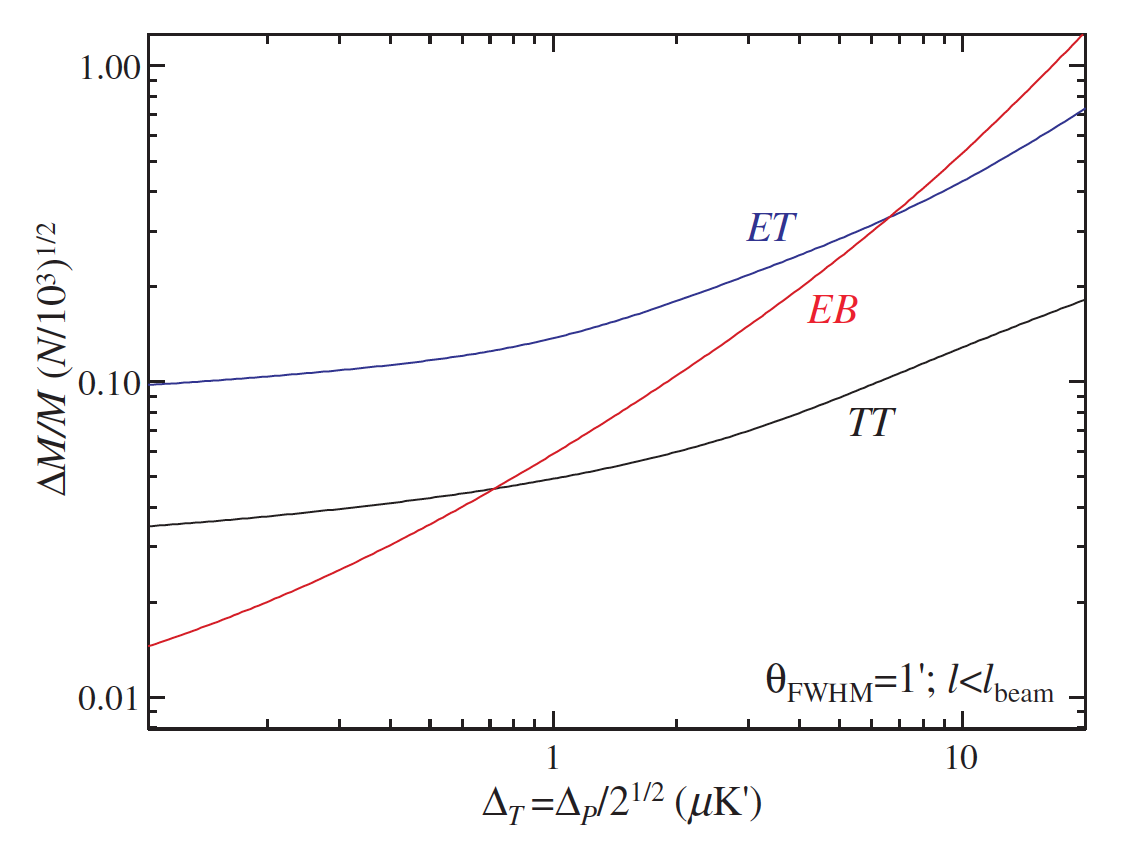
\includegraphics[width=0.95\textwidth]{CMBLensing/HaloLensing.png}
\caption{}
\end{figure}

CMB experiments have only very recently reached the resolution and sensitivity required to detect the lensing signal from dark matter halos, with recent measurements by ACTPol, SPT and Planck (cite) being the first. S4 will be capable of providing mass calibration for clusters that will be an independent confirmation of the mass scale (also obtainable from galaxy lensing) and will be indispensable for high-z clusters. An arcminute resolution experiment with a sensitivity of around 1$\mu$K-arcmin can determine the mass scale of 1000 high-z clusters to better than 4\% using temperature maps and independently to better than 5\% using polarization maps. The primary systematic in temperature is the thermal SZ effect; however this can be mitigated using multi-frequency information due to the spectral dependence of the tSZ effect. The kinetic component of the SZ effect can also be mitigated by utilizing information from the polarization estimators -- where the SZ contribution is expected to be small -- especially since polarization estimators offer comparable signal-to-noise at S4 sensitivity levels.

Useful plots: beam dependence of mass calibration uncertainty? beam dependence of number and mass of detected clusters? relative S/N from different polcombs of estimators?



\section{Delensing}\label{delens}

For noise levels below $\Delta_P \simeq 1 \mu$K-arcmin,  the dominant source of effective noise in $B$-mode maps is the fluctuation induced by the lensing of $E$-modes from recombination.  This signal has a well-understood amplitude, and unlike other sources of astrophysical fluctuation in the map, it cannot be removed with multifrequency data.  Instead it must be removed using map-level estimates of both the primordial $E$ maps and the CMB lensing potential $\phi$.

As discussed in the dedicated CMB lensing chapter, delensing will be a crucial portion of the reconstruction of the CMB lensing field, for science goals like measuring the neutrino mass.  This is because at low noise levels a quadratic reconstruction of lensing using the $EB$ estimator (Hu \& Okamoto 2001) can be improved upon by cleaning the CMB maps of the lens-induced $B$ fluctuationf and then performing lens reconstruction again.  CMB maps cleaned of the lensing signals will thus be produced as part of the CMB lensing analysis procedure.

Delensing can in principle be a perfect procedure, in the sense that in the limit of no instrumental noise or primordial $B$ modes, the lensing potential and the $E$ mode map can be perfectly imaged (Hirata/Seljak 2003).  However, the finite noise in a S4 survey will lead to residual lensing $B$ modes which cannot be removed and will act as a noise floor for studying B modes from tensors.  The amplitude of these residual lensed $B$ modes are discussed in the dedicated lensing chapter as a function of the angular resolution and the noise level of the S4 survey; in particular, it is crucial to have high-angular resolution maps in order to obtain the small-scale $E$ and $B$ fluctuations needed for the $EB$ quadratic lensing estimator.

The concerns with the delensing procedure are similar to those for measuring the lensing power spectrum. The impact of polarized dust and synchrotron emission from the Galaxy, and the impact of polarized point sources on small scales on the lensing reconstruction are addresed in chapter XX.

Additionally, rather than using an estimate of the CMB lensing field obtained from the CMB itself, it is also possible to use other tracers of large-scale structure which are correlated with  CMB lensing (Smith+ 2010).  In particular the dusty, star-forming galaxies that comprise the cosmic infrared background (CIB) are strongly correlated with CMB lensing, due to their redshift distribution which peaks near $z \sim 2$ (Sherwin+ 2014; Simard+ 2014).  The level of correlation is approximately $80\%$ (Planck 2013 XVIII) and can in principle be improved using multifrequency maps of the CIB which select different emission redshifts (Sherwin+ 2014). 

\begin{figure}[h]
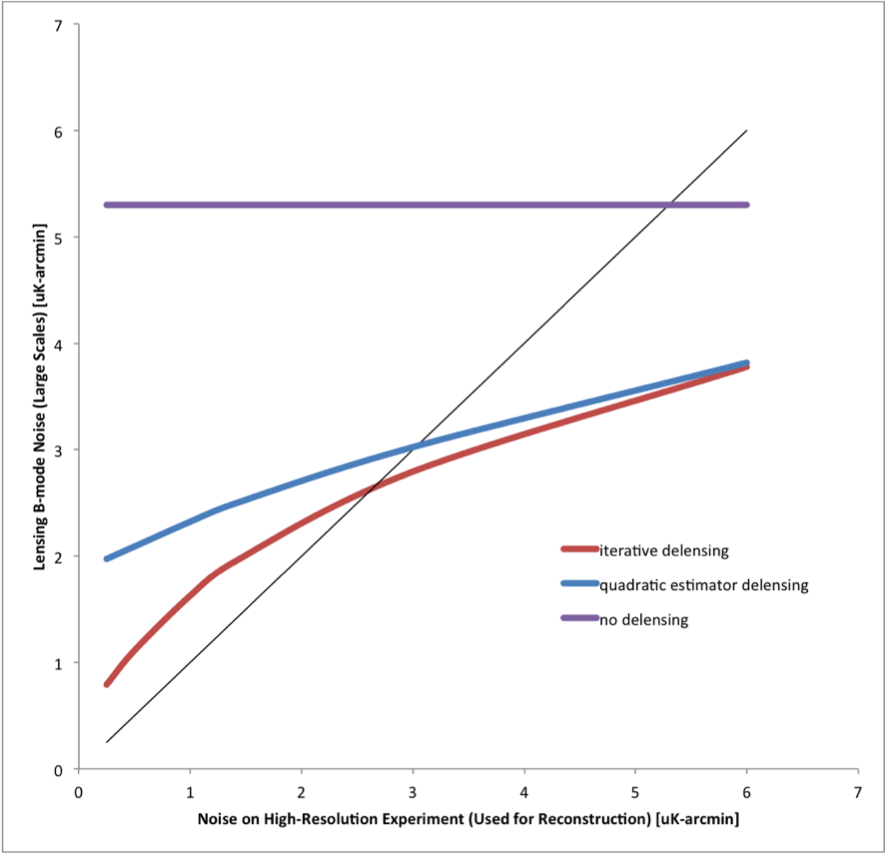
\includegraphics[width=0.75\textwidth]{CMBLensing/delensingIterative.png}
\caption{test}
\end{figure}



\subsection{Method}


\subsection{Parameter Forecasts with Delensing}\label{delensForecast}


\section{Systematic Effects and Mitigation}\label{syst}
The quadratic estimators used for lens reconstruction search for departures from statistical isotropy.  The lens effect locally changes the CMB power spectrum via shear and dilation effects (e.g. Bucher+2011).  Other sources of statistical isotropy can thus be confused with lensing effects; these can be of both instrumental and astrophysical origin.

\subsection{Astrophysical Systematics}
Extragalactic sources and SZ clusters in T maps.  Planck (2013) removed the effect of Poisson sources in the CMB four-point function from their lensing autospectrum which left untreated would have shifted their measured lensing power spectrum amplitude by $4\%$, a  1$\sigma$ shift.  For an experiment with lower map noise level and smaller beam, such as CMB-S4, sources can be found and removed to much fainter flux thresholds.  The largest sources of bias then come from the clustered, or correlated, portions of the four-point functions of the sources and the correlations with the lensing field.  These biases can be as large as several percent (van Engelen+2013, Osborne+2013) and their amplitude is highly model-dependent. 

These biases are inherent on the sky but can likely be mitigated using a combination of techniques, (1) making heavy use of multifrequency data; (2) projecting them out of the lensing estimate, an approach known as "bias-hardening" (Osborne+ 2013) (3) masking sources aggressively.

Galactic dust.  Four-point function of polarized dust??  (Let's measure this with Planck 353GHz data)

\subsection{Instrumental Systematics}
 	


What level of control do we need on these?

-gain variations, monopole leakage, quadrupole leakage, pointing/beam offsets

These can be estimated directly from the data using quadratic estimators (cite Yadav/Su/Zaldarriaga)


\section{Instrument, Survey, and Simulation Requirements}\label{require}

-effect of nonlin growth

 -- bias from 2nd order perturbations (tree level bispectrum) is 1\% for an S4 survey (Boehm+ in prep; Sherwin+ in prep).  

Is some information lost due to mode-coupling by nonlin growth (AVE comment, this should be pretty easy to answer)





%\bibliography{cmbs4}

%\end{document}

%%
%% Populate the .bib file with entries from SPIRES Bibtex (preferred)
%% or ADS Bibtex (if no SPIRES entry).
%%  SPIRES will also supply the CITATION line information; please include it.
%%

